%%%%%%%%%%%%%%%%%%%%%%%%%
\section{Use Cases} \label{useCases}
%%%%%%%%%%%%%%%%%%%%%%%%%
In this chapter some of the possible actions that can be performed into \applicationName\ are presented. The aim of this chapter is to provide a practical introduction to \applicationName, through different use cases.
\subsection{Access information}
The first use case presented introduces the available option to access building models data.\\
An InfoBox is shown, whenever a building is selected through a click of the mouse or a tap on the screen of a smartphone. Figure \ref{fig:infoBox} shows how these information are given to the user.
\begin{figure} [H]
\centering
\begin{subfigure}[b]{1\textwidth}
	\centering
	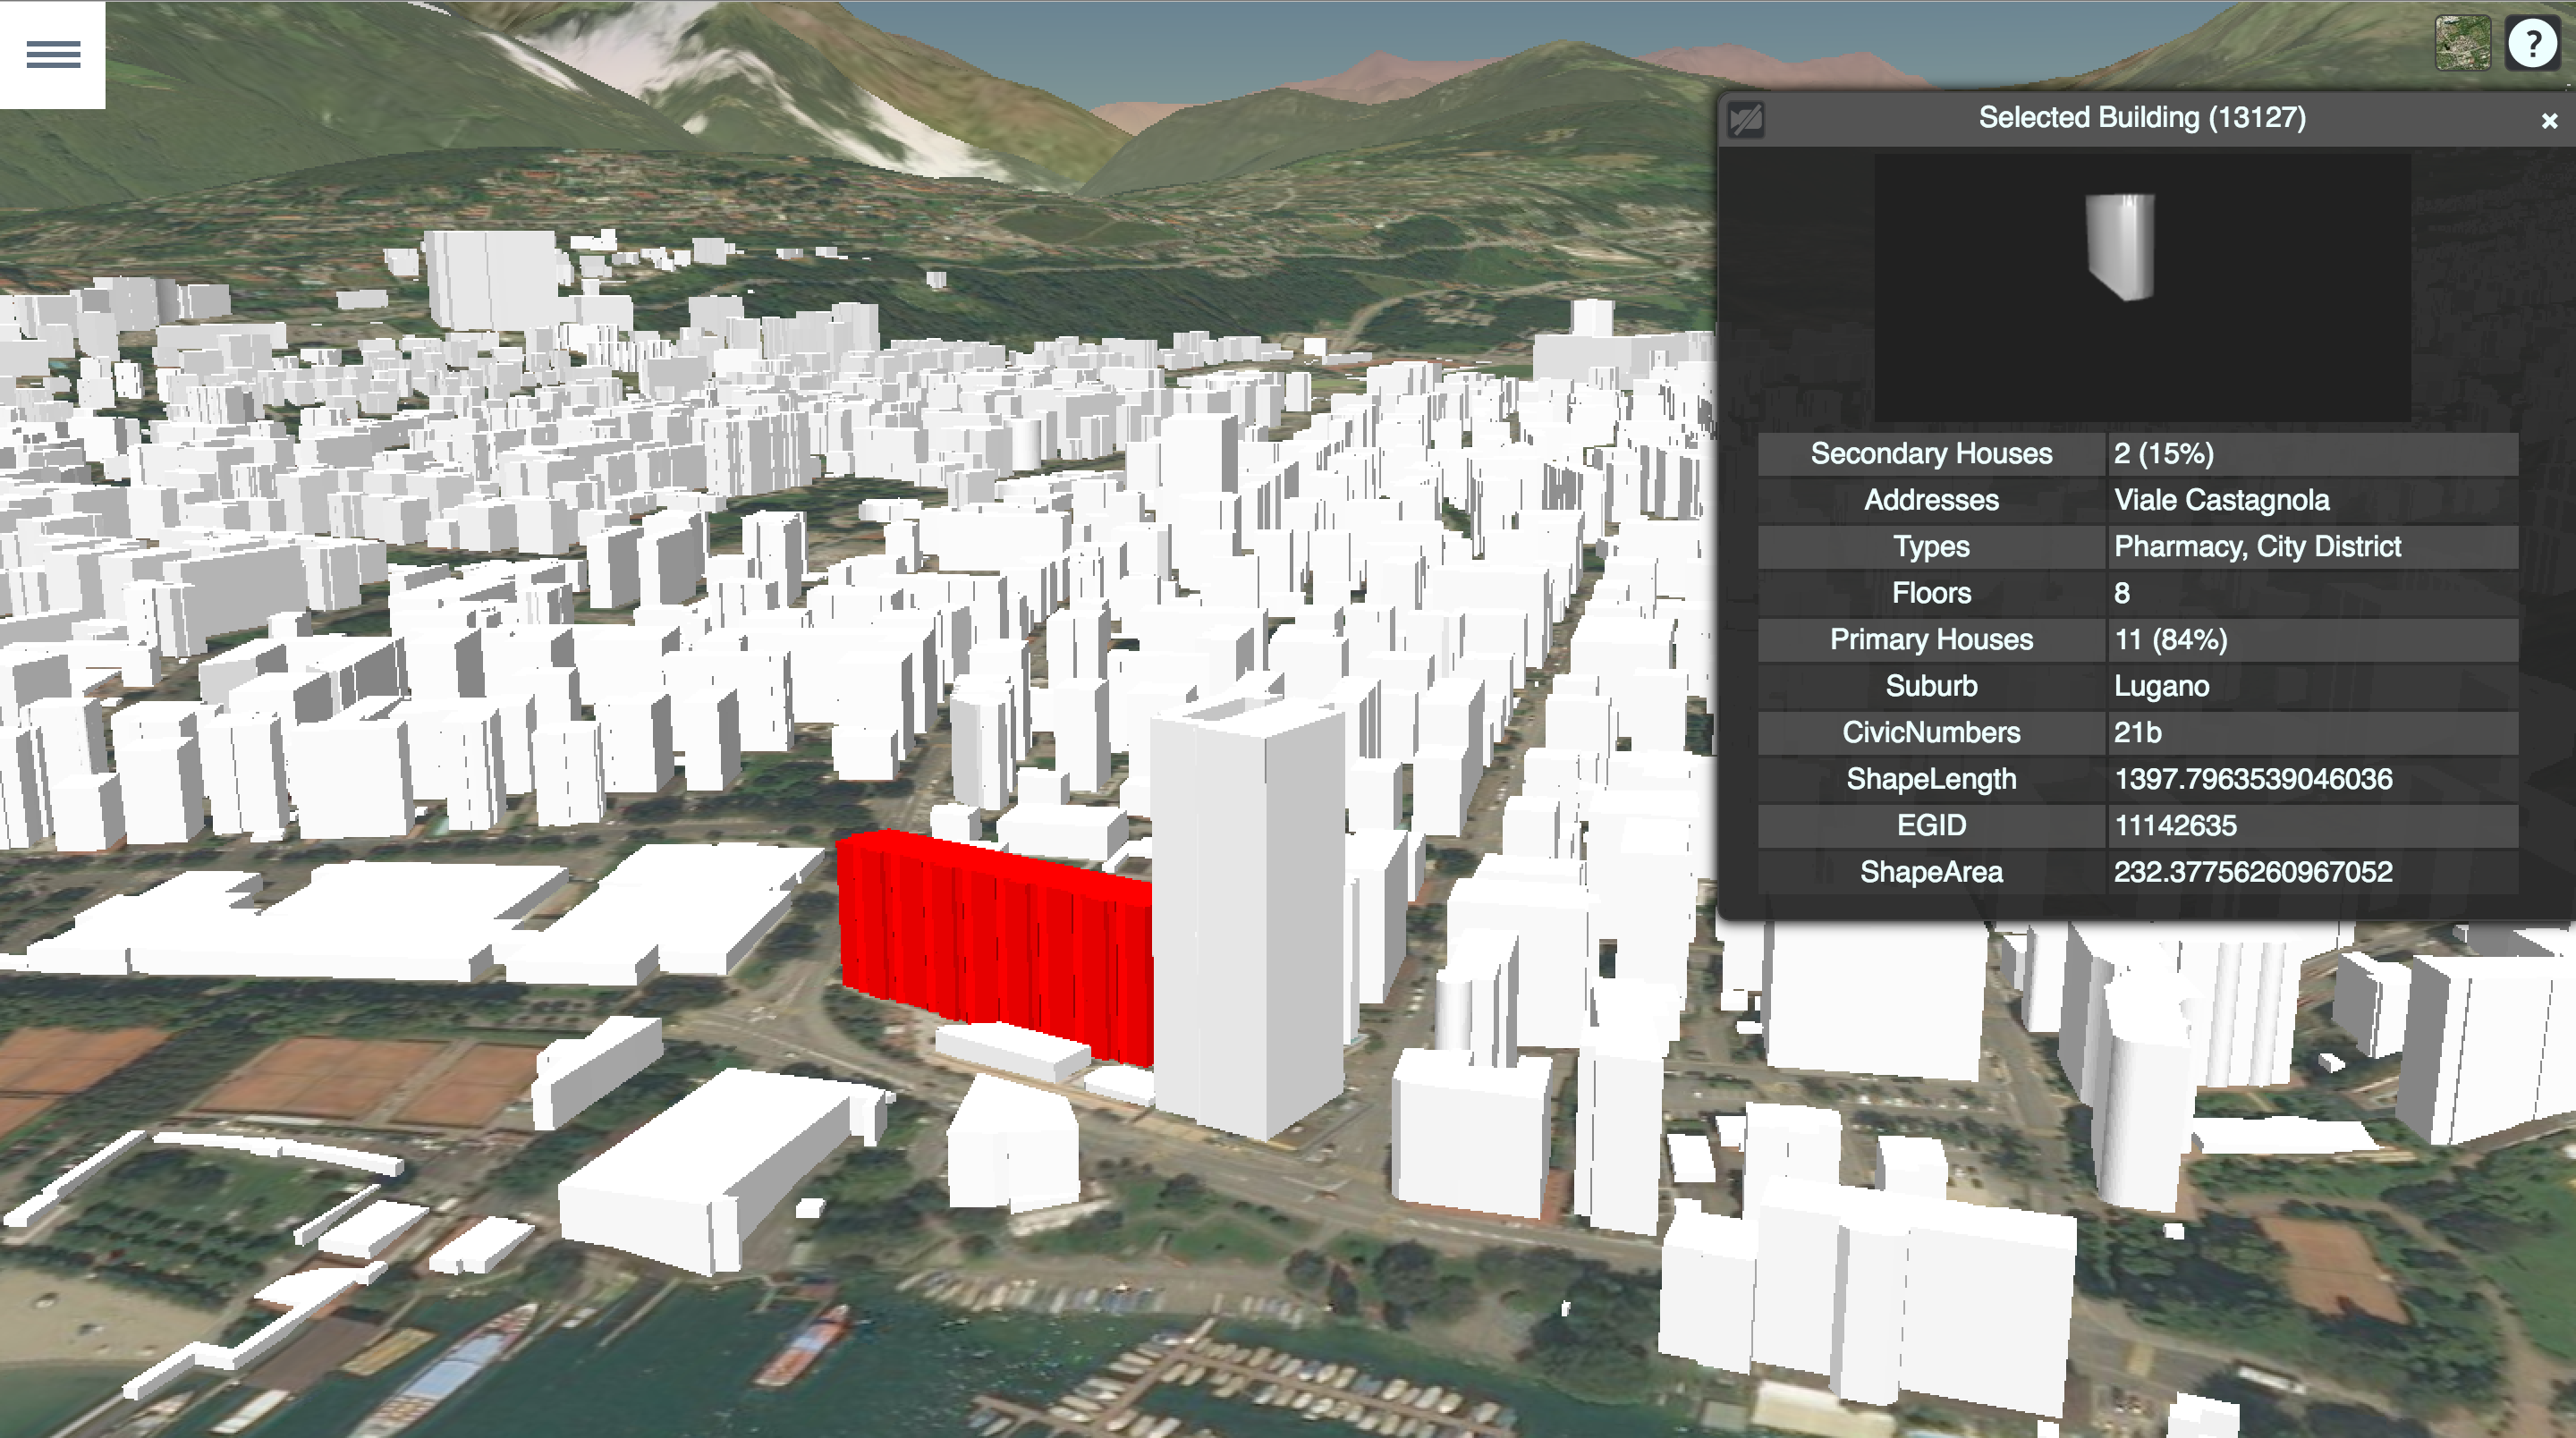
\includegraphics[width=0.8\textwidth]{chapter4/images/infoBox_city}
	\caption{Selecting a building will make the InfoBox appear automatically}
	\label{subfig:infoBox_city}
\end{subfigure}
\begin{subfigure}[b]{1\textwidth}
	\centering
	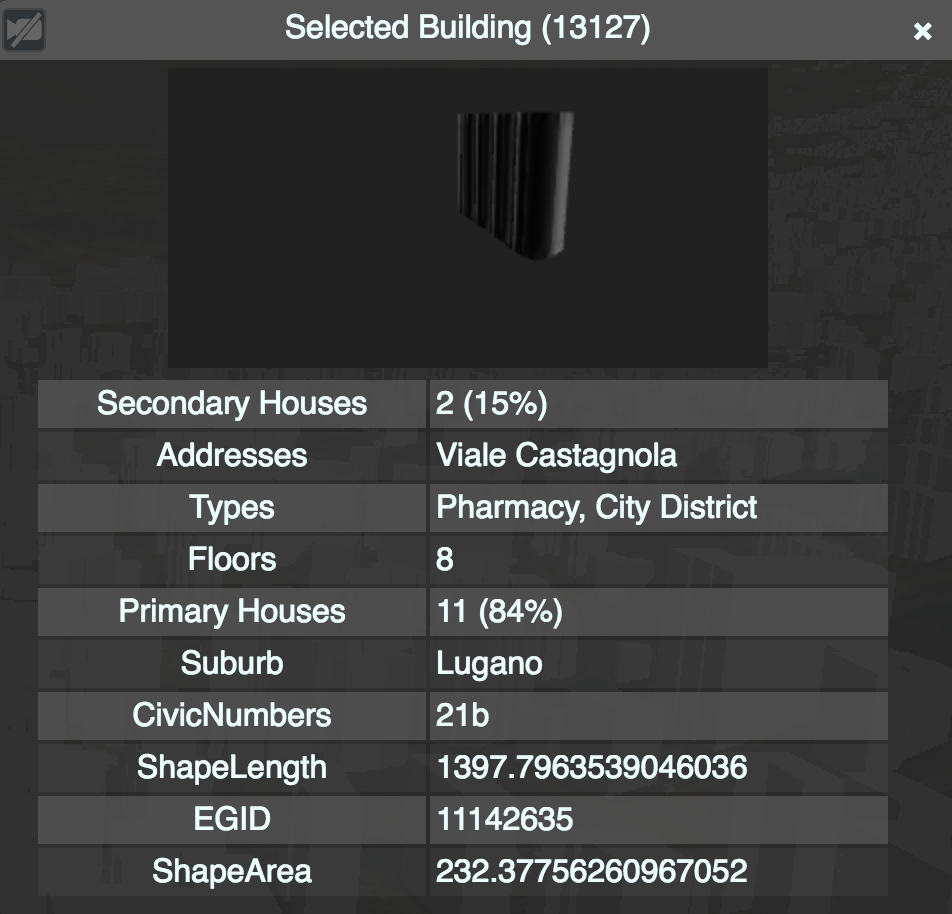
\includegraphics[width=0.7\textwidth]{chapter4/images/infoBox}
	\caption{A detailed look at the InfoBox}
	\label{subfig:infoBox}
\end{subfigure}
\caption{Accessing the information of buildings in \applicationName}
\label{fig:infoBox}
\end{figure}
The first field displayed is a 3D representation of the model of the building clicked without its surrounding environment. It is possible to interact with this canvas in order to rotate and zoom the building model freely.\\
After, a list of useful information about the building follows: the length of this list changes from building to building depending on the availability of the information.\\
The building clicked in the example of figure \ref{fig:infoBox} presents all the possible available information that an user can get about a building.\\
The fields of the displayed data are denoted as follows: 
\begin{itemize}
\item {\bf Types} provides the list of groups in which the building is present. Groups are defined by the OpenStreetMap APIs and are used to represent the usage of the buildings which, conceptually, have characteristics in common. Examples of types are: Post Office, Pharmacy, Hospital, University etc \dots.
\item {\bf Floors} is the number of floors that the building possesses
\item {\bf Shape Length \& Shape Area} represent the size of buildings available for consultancy, they are measured in length and area both expressed in meters.
\item {\bf Street Name \& Civic Numbers} are the data concerning the addresses of the street where the building is located. There could be more than one street name and civic numbers in case the building has many of them (e.g., different entrances in the same building that are on different streets). Addresses data are taken from Swisstopo APIs and, if not available from this service, OpenStreetMap APIs are used.
\item {\bf EGID} the unique identifier of the building given by the Swiss REA 
\item {\bf Suburb} represents the suburb in which the building is located
\item {\bf Primary \& Secondary houses} represents both the number of primary and secondary houses in the selected building and the percentage that each value represents over the total number of houses in that building
\end{itemize}

\subsection{Visualize the City}
\begin{figure} [H]
\centering
\includegraphics[width=0.9\textwidth]{chapter4/images/application_bySuburb}
\caption{A Visualization of the city of Lugano where every suburb is coloured differentrly}
\label{fig:application_bySuburb}
\end{figure}
\subsection{The Query System}
\subsubsection{Building Selection}
\subsubsection{City Gradient Map}